\documentclass[10pt]{scrartcl} 

\renewcommand{\baselinestretch}{1.15} 

\usepackage[english]{babel}
\usepackage[utf8]{inputenc}  

\usepackage{import}
\usepackage[smaller]{acronym}
\usepackage[export]{adjustbox}


\usepackage{geometry}
\geometry{a4paper,left=30mm,right=30mm,top=25mm,bottom=35mm}                    

\addtolength{\topmargin}{-1.0cm}
\addtolength{\paperheight}{10pt}
\addtolength{\textheight}{+2.5cm}
 
\begin{document} 

\title{Initial Report on Raytracing}
\author{Team Raytrashing}
\date{February 2018}

\maketitle

\section{Aims}
Our main aim as a team is to implement a working Raytracer with an efficient back-end coupled with a user-friendly front-end. We also intend to learn new software, technologies and tools (like Python, JavaScript, TravisCI etc.) as a part of this project and we want to do so by working together as a team. 
As far as the specific technical aims of the project are concerned, we wish to implement a raytracer with the following features and their priorities/levels given in the brackets (1 being the highest priority on a scale of 10):
\begin{itemize}
    \item Diffusion and Specular Reflection (1)
    \item Shadows (1)
    \item Rendering multiple shapes like sphere, cube, pyramid etc. (1)
    \item Translucency (2)
    \item Reflection (2)
    \item Ability to render the shapes within 30-40 seconds (2)
    \item Responsiveness on the front-end (2)
    \item Client-Server Architecture (3)
    \item Multi-Threading for faster performance (3)
    \item Drag and Drop capability on the front-end (4)
    \item Making the website secure - HTTPS (5)
    \item Ability to change the camera position (6)
    \item Saving the current scene for future reference (6)
    \item Distributed Systems for faster performance (8)
    \item Live-rendering using thumbnails (9)
\end{itemize}
We wish to implement these by continuously referring to the milestone plan by keeping in mind the priorities of each task.


\section{Strategy}
Our team convened to discuss which technologies to use for the Raytracer implementation and during the first meeting, we had decided to use Python and Django for the back-end and JavaScript coupled with HTML and CSS for the front-end. The reason to choose Python and JavaScript for the development was because none of us had previously extensively worked on either of the technologies and we thought this is a good opportunity to learn and hone our skills in these languages. We also decided to implement a Client - Server architecture to integrate the front-end and the back-end. The output of the front-end is a JSON file, which is then sent to the back-end using an HttpRequest. Subsequently the back-end renders the scene and sends the image back to the front-end, so it can be displayed to the user.\par
Our strategy is also to reduce the number of bugs we have to deal with and hence we have accepted that our development will follow Test Driven Development (TDD) and Pair Programming. We are following TDD by creating test cases and then developing so that we can reduce the number of bugs. Pair programming also helps in avoiding buggy code. \par
As a team, we also decided that we would be using the Agile methodology for our software development. We are following weekly Sprint cycles and we convene on Tuesdays from 13:00 to 16:00 by booking a room with the help of King's Venues.
We use Trello boards for maintaining the tasks and keeping track of them and during the weekly meetings, we accept previous sprint's tasks and define new tasks for the upcoming sprint. We also have a Trello board to keep track of every bug detected, in order to be able to prioritise them and fix them as soon as possible.


\section{Milestones - Timetable}
During our meetings, we created a timetable with milestones. Each milestone is directly linked to the sprint goals of each week. Of course, delays can occur and tasks may get pushed by a week, but we have also accounted for that, by having a lot of extra time at the end to fix any bugs or issues that may come up.
\begin{figure}[h]
\centering
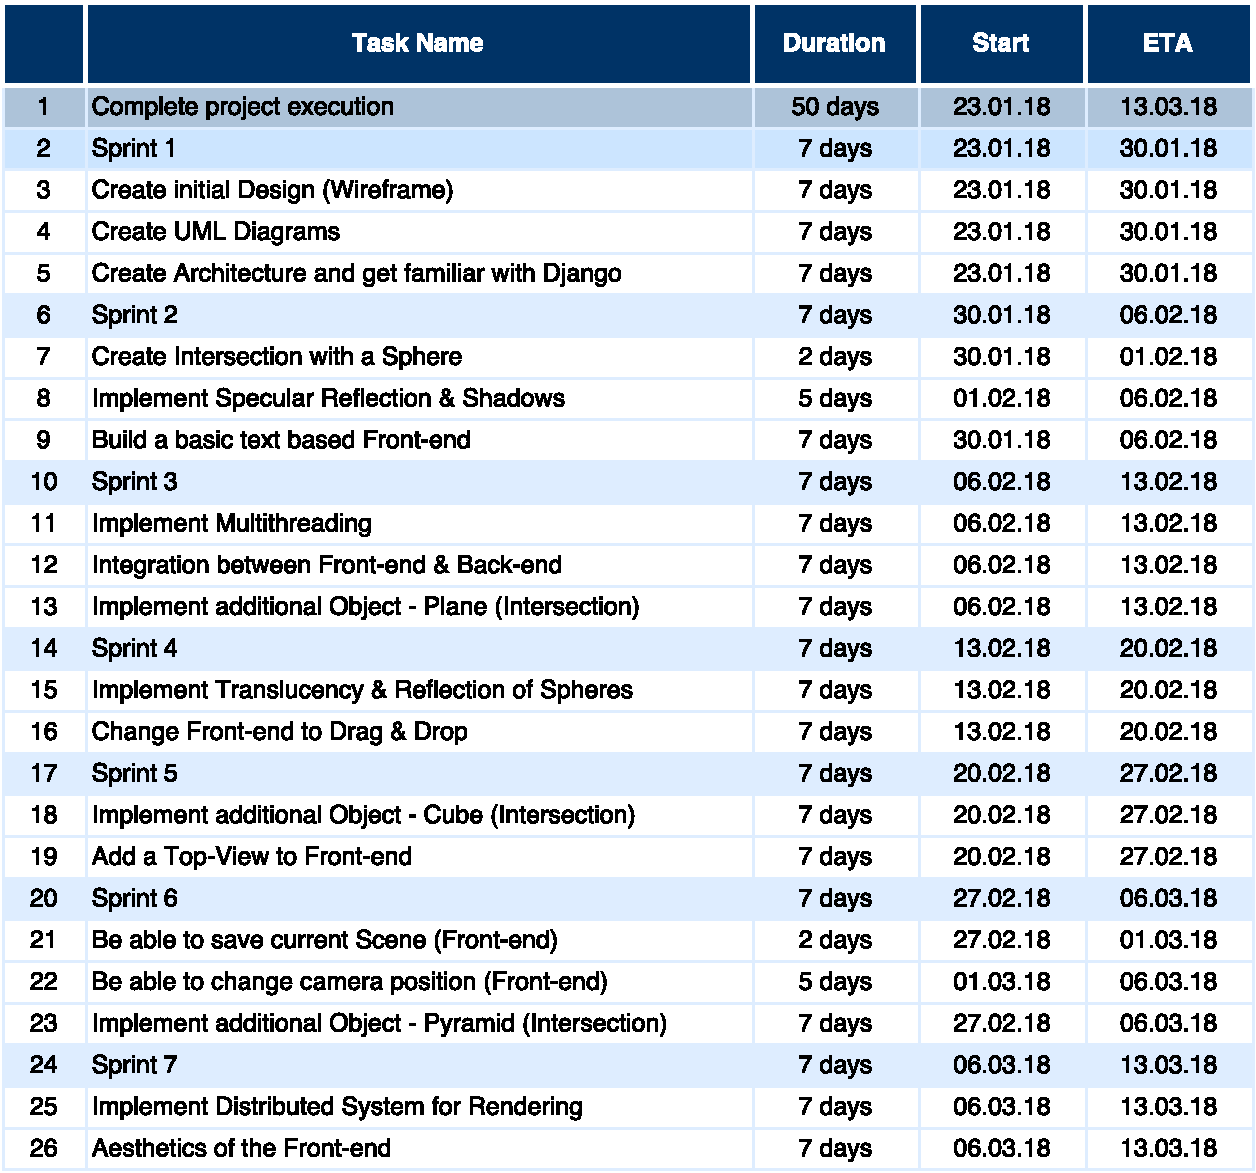
\includegraphics[width=0.8\textwidth]{images/time_table.pdf} % To change the image size, change the factor 0.8
\caption{Project Time Table} 
\label{fig:TimeTable} 
\end{figure}

\section{Initial Progress}
Initially, we did face some problems with the communication among the team members. Some minor confusion ensued in the first week but everything got back on track after everyone got accustomed with the tools and the technologies. We, as a team, got familiar with GitHub and the nuances of it like feature branches and pull requests. We have put in a lot of effort till now and just within two weeks of the start of the group project we have a working front-end and back-end and we are ready with a basic prototype. We are on track with what we set as milestones in the milestone plan and the aims of the project.


\section{Project Organisation}

\subsection{Team-organization}

At the moment three people are working on the front-end and the other three people on the back-end. But after a few weeks we will have rotations, meaning that one person from the front-end team will trade places with one developer from the back-end. This will help us to get a different, fresh view on the software, because after working a long time on the same part, it is possible, to become \grqq{}tunnel-visioned\grqq{}.

\subsubsection{Processes}

To achieve a good collaboration and integrate everyone of the team we are using two main approaches for the software development process.

\paragraph{Pair Programming}

According to the principle: Two heads are better than one, we are sometimes developing in pairs. This helps us to discuss thoughts and opinions, while writing the code. Furthermore, the probability to overlook a mistake decreases. In the end, the software contains less bugs.

\paragraph{Test Driven Development}

Testing a software product is one of the most important steps during the development. To improve the code quality we try to reach a very high code coverage. TDD helps us to achieve this;  we first write the tests and then implement the functionality. Moreover, the person who implements a feature does not write the tests for it. 

\subsubsection{Tools}

As a support for the aforementioned processes, we are using different software tools.

\paragraph{Slack}

For the main communication we are using the collaboration tool Slack. One of the most important features is the usage of different channels to separate unrelated topics. Our essential channels are: Back-end, Front-end, Announcements, Documentation and General (channel for general topics).

\paragraph{Trello}

As described above, we are using the scrum framework as an Agile strategy for the software development process. Trello is our scrum board, where we manage our user stories. A user story transitions through multiple states. At the beginning, a user story is defined and added to the general backlog. Then it is assigned to a developer and moved to the sprint backlog. During the sprint s/he will move it to the state \textit{in progress} and then to \textit{verifying}. Finally, if the implementation passes the tests and reviews, the user story is moved to \textit{done}.

\paragraph{Travis CI}

Since we follow the approach of Test Driven Development, we have a very good code coverage and hence, a lot of tests. In the next few weeks, the number of tests will increase and running all the tests manually is time consuming. Travis runs the whole list of tests automatically, as soon as it recognizes a push to the repository. 
\\
Furthermore, Travis CI helps us to find bugs before a pull request gets merged. If the manual code review was successful, it is still possible that a test is deemed unsuccessful. As a result Travis CI will block the merging and request changes. Especially during the refactoring progress, these automated tests are really helpful. 

\paragraph{Skype}

If we are unable to meet in person, we use Skype for pair programming and communicating. The advantage is, that even if it is late in the evening, we can start a pair programming session. 

\subsection{Peer-Assessment}

We discussed different possibilities, to handle the final peer assessment. To make it fair and uninfluenced we decided to use a anonymized scoring method, that gets described in detail in the next session.

\subsubsection{Method}

The mechanism we are using for the peer assessment allows each team member, to score the other members anonymously. This helps to avoid influenced decisions, because a person may not have the courage and self-awareness to express his opinion. To get a clear understanding how the proposed method works we will look at an example.

\paragraph{Example}

A student team TrashingRay with the four members, Alice, Bob, Charlie and David, is using the given assessment method. 

\begin{enumerate}  
\item Every team member has a total of 100 marks, which has to be distributed and assigned among himself and the other members. Alice, for e.g., may assign herself 30, Bob 24, Charlie 25 and David 21 points. 
\item Let's assume Alice received the following points: 30, 30, 26, 24. To avoid a situation where a person assigns himself a very high or a person he doesn't like, a very small number of points, the points for each individual are sorted and the highest and lowest values are deleted. 
\item For each person the average of the remaining points is calculated. In Alice's case this is the average of 30 and 26. 
\item As a result of the deletion, it is possible that some points get \grqq{}lost\grqq{}. In this example, we assume that the sum of marks is only 99 and one point is missing. To compensate this, the remaining points (in this case, 1), is distributed equally to all team members 
\end{enumerate}



\subsubsection{Solving Conflicts}

Of course it could be possible that some team members are not happy with the result of the peer assessment. If at least two people are not satisfied, we will start an open discussion. This should help to clarify why they think their marks are too low.  If necessary, a second round of voting could occur to end the deadlock.


\end{document}